\documentclass[../../../../main.tex]{subfiles}
\begin{document}

\begin{flushright}
\footnotesize\textit{【自動文字起こし・要確認】}
\end{flushright}

[解] $A(1,0), X(c,s) \ (c=\cos\theta, s=\sin\theta)$
$(0 \le \theta < 2\pi)$ とおいて良い。
点$X$の位置ベクトルを$\vec{x}$と表す。

\begin{center}
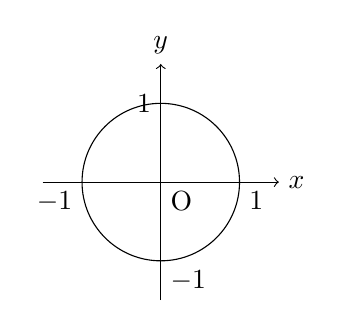
\begin{tikzpicture}
\draw[->] (-1.5,0) -- (1.5,0) node[right] {$x$};
\draw[->] (0,-1.5) -- (0,1.5) node[above] {$y$};
\draw (0,0) circle (1);
\node[below right] at (0,0) {O};
\node[below left] at (-1,0) {$-1$};
\node[below right] at (1,0) {$1$};
\node[below right] at (0,-1) {$-1$};
\node[left] at (0,1) {$1$};
\end{tikzpicture}
\end{center}

(1) $\vec{y} = \begin{pmatrix} 1 \\ 0 \end{pmatrix} - 2\begin{pmatrix} 1 \\ 0 \end{pmatrix} \cdot \begin{pmatrix} c \\ s \end{pmatrix} \begin{pmatrix} c \\ s \end{pmatrix}$ \\
$ = \begin{pmatrix} 1 \\ 0 \end{pmatrix} - 2c\begin{pmatrix} c \\ s \end{pmatrix}$ \\
だから \\
$|\vec{y}|^2 = (1-2c^2)^2 + 4c^2s^2 = 1 \quad \therefore |\vec{y}|=1 \ (\because |\vec{y}| \ge 0)$ \\
より、$|\vec{y}| = 1$ \hfill(終)

(2) $\vec{y} = -\vec{a}$の時、\\
$\begin{pmatrix} 1-2c^2 \\ -2cs \end{pmatrix} = \begin{pmatrix} -1 \\ 0 \end{pmatrix}$ \\
$\therefore c=\pm 1, cs=0$ \\
$\therefore (c,s) = (\pm 1, 0)$ \\
だから、$X=A$ 又は $A$と$X$を結ぶ直線と円の交点のうち、$A$でない方 \hfill(終)

(3) $Y(X,Y)$とおく。\\
$X = 1-2c^2 = -\cos 2\theta$ \\
$Y = -2cs = -\sin 2\theta$ \\
だから、$\theta$が$0 \le \theta < 2\pi$でうごくとき、$Y$は$C$を2回まわる \hfill(終)

\end{document}
